\begin{comment}
 
\begin{frame}{A path with many options}
 \begin{itemize}
  \item There are many different options to choose
  \item I explain my choices but discuss other options
  \item Goal: Be clear so other researchers can adapt my methodology to their problems
 \end{itemize}

\end{frame}

\begin{frame}{MI primer}
\begin{itemize}
 \item MI forms the base of this thesis
 \item There are lots of different ways to impute
 \item As long as we can impute valid imputations, we can analyze them
 \item Poor imputation leads to poor results (bias, variability, loss in power)
\end{itemize}
\end{frame}

\end{comment}

\begin{frame}{MI Notation}
 
 \begin{itemize}
\item $Y$ is our whole dataset. It will have $i$ rows and $j$ columns. Some of the covariates in the dataset will be completely observed, and others will have missingness.
\item $Y_j$ is a specific column of Y. $Y_j$ is composed as $Y_j=(Y_{j,obs},Y_{j,mis})$, where
	\begin{itemize}
	\item $Y_{j,obs}$ is the data we have observed for covariate j
	\item $Y_{j,mis}$ is the missing data covariate j
\end{itemize} 
\item $Y_{obs}$ is all of the data that we have observed
\item $Y_{mis}$ is all the data that we have not observed
\item R is a binary matrix the same size as $Y$ where a 1 indicates we observed the data, and 0 means it is missing
\item $\psi$ is a vector of parameters for the missing data model. 
\item The missing data model is given as $p(R|Y_{obs},Y_{mis},\psi)$
\item $\theta$ is a vector of the parameters for the full model of $Y$
\item $\phi_j$ is the unknown parameters of the imputation model 
\end{itemize}
\note{Missing data model relates Y to R}
\end{frame}

\begin{comment}
\begin{frame}{MI Concepts}
\begin{itemize}
 \item Ignorability
$$p(Y_{mis}|Y_{obs},R)= p(Y_{mis}|Y_{obs})$$
That is, we may ``ignore'' the R. The probability of the data being missing does not depend on how the data is missing. 
Equivalently, we may write this as
$$p(Y_{mis}|Y_{obs},R=1)= p(Y_{mis}|Y_{obs},R=0)$$
\item Non ignorability: $$p(Y_{mis}|Y_{obs},R=1)\neq p(Y_{mis}|Y_{obs},R=0)$$
So we must take into account the missing data structure for imputation.


\end{itemize}

\note{Being ignorable makes it justified to model our missing data from our observed data, without needing to worry about how it was missing.
The opposite of ignorable data is called non-ignorable data, in this case.
We often times see ignorable missing data in practice,
although one should certainly check the sensibility of ignorability, as some instances will certainly be non-ignorable, 
for example censored data, or when we know that the missing data is systematically different than the observed. 
If we have strongly nonignorable data, we should either try one of two things.

The first is to expand the data (collect something else similar to the covariate with missingness) so that it becomes ignorable and 

the second is to formulate two imputation models, one for the observed and one for the missing.

}

\end{frame}

\end{comment}

%666 moving this to intro
\begin{frame}{Missing data Mechanisms}
Now, we may discuss the three main types of missing data mechanisms. 
\begin{itemize}

\item MCAR: Missing completely at random:  $$P(R=0|Y_{obs},Y_{mis},\psi)=P(R=0|\psi)$$
\begin{itemize}
\item The missingness in the data is not at all related to any of the data that we do or don't have
\end{itemize}
\item MAR: Missing at random: $$p(R=0|Y_{obs},Y_{mis},\psi)= p(R=0|Y_{obs},\psi)$$
\begin{itemize}
 \item The missingness we have is related to something in the data 
\end{itemize}
\item MNAR: Missing not at random: $$p(R=0|Y_{obs},Y_{mis},\psi)$$ does not simplify
\begin{itemize}
 \item  and the missingness depends on data that we have as well as have not collected
\end{itemize}
\end{itemize}
\note{
 If a lab technician slips and drops 5 vials of blood, the missingness caused by this would be MCAR
 If we collect the gender of the subject and we know that males tend to not give blood, we can attribute the missingness to the gender. In general, MAR models are ignorable.
 For example if a full moon causes the blood testing machine to break more often, but we don't have the moon phase as a variable.
}
 
\end{frame}

%JM was here

%moved this to intro 666
\begin{frame}{Full Conditional Specification (FCS)}
 \begin{itemize}
  \item Assume MAR missing data mechanism %although MNAR with more 
  \item Missing data is imputed iteratively on a variable by variable basis
  \item Drawing from $p(Y,R|\theta)$ through the full conditionals $p(Y_j|Y_{-j},R,\theta_j)$
  \item Requires no distributional assumptions
  \item Idea: Specify k one dimensional models to impute on the missing data columns
 \end{itemize}

\end{frame}

%moved this to intro 666
\begin{frame}{FCS Algorithm}
  \begin{figure}[h!]
  \centering
    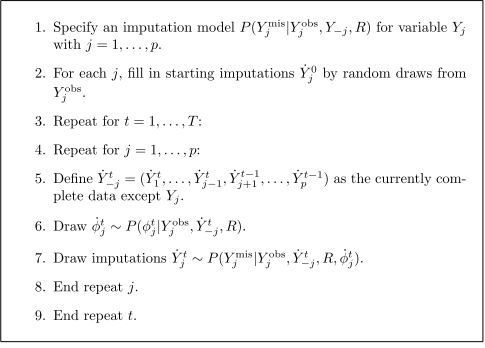
\includegraphics[width=0.6\textwidth]{fcs_algo}
  \caption{FCS imputation pseudocode, taken from \cite{VanBuuren2012}}
\label{fig:fcsexample}
\end{figure}
 \note{ Observe how the previous imputation Y_j^(t-1) only enters the current imputation
 through its relation with other variables, and not directly. This makes convergence very fast
}
\end{frame}

%moved this to intro 666
\begin{frame}{FCS Pros and Cons}
Pros
 \begin{itemize}
  \item Flexible
  \item Easy to specify models
  \item Handles mixed continuous categorical
 \end{itemize}

 Cons
 \begin{itemize}
  \item No guarantee that full conditionals are compatible
  \item Slow
  \item Gets much harder as sample size increases to specify models
 \end{itemize}

\end{frame}

\begin{comment}
 
\begin{frame}{Decision}
 \begin{itemize}
  \item Both are not as good as having complete data
  \item Cancer and survival data present challenges for JM
  \item FCS offers us the most ease and flexibility
 \end{itemize}
\end{frame}

\end{comment}

\begin{frame}{Setting Up The Model}
\begin{itemize}
 \item Specify the models
 \item Specify the predictors for each model
 \item Determine number of iterations and datasets to impute
 \begin{itemize}
  \item This is a topic of hot debate
  \item Old literature suggested 5 imputations, 5 iterations, but more now
 \end{itemize}

\end{itemize}

\note{Many disagreements, but all say at least 5}
\end{frame}

\begin{frame}{Checking The Imputations}
 Convergence
 \begin{itemize}
  \item Chains should be freely intermingled with no pattern
  \item Convergence when variance between chains is no larger than variance within each chain
  \item Formal tests like Gelman/Rubin $\hat{R}$ proposed to check convergence
 \end{itemize}
Validation
\begin{itemize}
 \item ``Does the data look like it could have come from real data had it not been missing''?
 \begin{itemize}
  \item Requires intimate knowledge of the data
 \end{itemize}
\item Graphical checks
\begin{itemize}
 \item Density plots
 \item Conditional scatter plots
 \item Box and whisker
 \item etc.
\end{itemize}

\end{itemize}
\end{frame}

\begin{frame}{Pooling}
 \begin{itemize}
  \item We now have $m$ imputed datasets
  \item Run the analysis on each of the $m$ complete datasets
  \item But we want one analysis, not $m$
 \end{itemize}

\end{frame}

%moved to intro 666
\begin{frame}{Rubin's Rules}
 Let
 \begin{itemize}
  \item $\hat{Q}_i$ be the scientific estimand from the $i^{th}$ MI dataset
  \item $U_i$ be the variance-covariance matrix of the $i^{th}$ MI estimand
 \end{itemize}
Then
\begin{itemize}
 \item The MI estimate is given by
 $\bar{Q}=\frac{1}{m}\sum_{i=1}^{m}\hat{Q}_i$
 \item The MI ``within'' variance is given by
 $\bar{U}=\frac{1}{m}\sum_{i=1}^{m}U_i$
 \item the MI ``between'' variance is given by
 $B=\frac{1}{m-1}\sum_{i=1}^{m}(\hat{Q}_i - \bar{Q})(\hat{Q}_i - \bar{Q})'$ % matrix notation?
   \item Total variance given by \cite{Rubin1987}
  $$T=\bar{U}+B +\frac{B}{m}$$
\end{itemize}

\end{frame}

%moved to inro 666
\begin{frame}{Inference with Rubin's Rules}
 \begin{itemize}
  \item Assume that with complete data, inference on the estimand
  Q would be based on the statement $(Q- \hat{Q})\sim N(0,U)$
  \begin{itemize}
   \item $\hat{Q}$ is the statistic estimating Q
   \item $U$ is the variance-covariance of $(Q-\hat{Q})$
  \end{itemize}
%    \item Since true T is not known, then
  $$\frac{Q-\hat{Q}}{\sqrt{T}}\sim t_{\nu}$$
  \item $\nu$ is given by \cite{Barnard1999}
  $$\nu=\frac{\nu_{old}\nu_{obs}}{\nu_{old}+\nu_{obs}}$$
\item Where $\nu_{obs}=\frac{\nu_{com}+1}{\nu_{com}+3}\nu_{com}(1-\frac{B + B/m}{T})$
\item $\nu_{com}$ is the hypothetical complete sample degrees of freedom
\item $\nu_{old}=\frac{m-1}{(\frac{B + B/m}{T})^2}$ 
 \end{itemize}

 \note{Requires normality
if not normal, transform}
\end{frame}


%stack method was here
